\documentclass{llncs}

% ======= Packages ======
\usepackage{etex}
%    ### General ###
%\usepackage{latexsym}
\usepackage{enumerate}

\usepackage{amssymb,amsmath}   %
%\usepackage{amsthm} % theorem environment

%    ### Format ###
%\usepackage{a4wide}     %% wide page
%\usepackage{times}      %% small fonts
%\usepackage{fullpage} 


%    ### Logic and Theoretical Computer Science ###
\usepackage{stmaryrd}
\usepackage[all, knot]{xy}%%xy-pics
\usepackage{verbatim}
\usepackage[english]{babel}
\usepackage{graphicx}

\usepackage[table]{xcolor}

%    ### Game Theory ###

%\usepackage{xspace}
%\usepackage{tikz}                %avoid multiple call !!
  %\usetikzlibrary{arrows,shapes,automata,backgrounds,petri,fit,decorations.pathmorphing}

%\usepackage[active,tightpage]{preview}
%\PreviewEnvironment{tikzpicture}
%\setlength\PreviewBorder{5pt}

%\usepackage{lgcommands}
\usepackage{tikz,subfigure}
   \usetikzlibrary{shapes.geometric}
\usepackage{pgfplots}
%    ### Linguistics ###
%\usepackage{tipa}   % International Phonetic Alphabet

%\usepackage{qtree}              %basicly   qtree and tikz-qtree do the samething
%\usepackage{tikz}                  % avoid multiple call !!
%\usepackage{tikz-qtree}            

%\usepackage{gb4e}         % NOTE!!!   This should be the LAST  usepackage   call!!!!!!!
%\usepackage{lingmacros}

%%% Micha's stuff
\usepackage{booktabs}
\usepackage{todonotes}

% ======== Definitions ========

\newcommand{\intp}[1]{\llbracket #1 \rrbracket}         %interpretation


% ======== Title ========

\title{Variations on a Bayesian Theme: Comparing Bayesian Models of
  Referential Reasoning} \titlerunning{Variation on a Bayesian Theme}
\author{Ciyang Qing \and Michael Franke\thanks{We are indebted to
    Judith Degen, Michael C.~Frank, Noah D.~Goodman and Daniel
    Lassiter, two anonymous reviewers, and the audience of the
    ESSLLI workshop ``Bayesian Natural Language Semantics and
    Pragmatics'' for stimulating feedback and discussion. Many thanks
    also to Henk Zeevat and Hans-Christian for organizing mentioned
    workshop, and to Will Frager for help accessing Amazon Mechanical
    Turk. Michael Franke gratefully acknowledges financial support by
    NWO-VENI grant 275-80-004.}}  \institute{Institute for Logic, Language and
  Computation\\Universtity of Amsterdam, The Netherlands}


% ======== Content ========

\begin{document}

\maketitle

\begin{abstract}
  Recent developments in Bayesian experimental pragmatics have
  received much attention. The Rational Speech Act (RSA) model
  formalizes core concepts of traditional pragmatic theories
  quantitatively and makes predictions that fit empirical data
  nicely. In this paper, we analyze the RSA model and its relation to
  closely related game theoretic approaches, by spelling out its
  \emph{belief}, \emph{goal} and \emph{action} components. We
  introduce some alternatives motivated from the game theoretic
  tradition and compare models incorporating these alternatives
  systematically to the original RSA model, using Bayesian model
  comparison, in terms of their ability to predict relevant empirical
  data. The result suggests that the RSA model could be adapted and
  extended to improve its predictive power, in particular by taking
  speaker preferences into account. 
\end{abstract}

%%%%%%%%%%%%%%%%%%%%%%%%%%%%%%%%%%%%%%%%%%%%%%%%%%
\section{Introduction}

Human language communication is efficient, in that people need not always say every detail in order to be understood. Rather, speakers only say what is most relevant, and listeners can seemingly effortlessly grasp the intended meaning beyond what is literally said. This ability to do pragmatic inference has been long studied and the \emph{conversational implicature} theory by Grice \cite{Grice} is one of the most prominent theories in the field. However, since it is hard to formalize the \emph{Cooperative Principle} and the \emph{Conversational Maxims}, Grice's theory is not precise enough to give empirically testable predictions, especially quantitative predictions.

The Bayesian \emph{Rational Speech Act} (RSA) model attempts to address this issue by using information-theoretic notions together with the Bayesian inference framework. It has been shown that the model could yield quantitative predictions that are highly correlated to actual human judgments \cite{Frank}.

Despite the RSA model's theoretical advantage in that it provides us with quantitative predictions and its empirical success, if we analyze the design of the model, we will find several choices that are not \emph{prima facie} obvious and thus need further clarification. These choices have their alternatives in the closely related game-theoretic approaches to pragmatics (e.g. \cite{Benz2007,Jager2013}), which have similar but slightly different conceptual motivations. Hence it is important to systematically compare the original RSA model with all these alternatives and test their predictions on empirical data, to gain a better understanding of the nature of human pragmatic inference.

The outline of the paper is as follows. We first introduce the simple referential communication game investigated in \cite{Frank} and the original RSA model proposed there. We then analyze a few design choices in this model and introduce their alternatives in game-theoretic pragmatics. Next we report the result of an experiment similar to the original one, and compare the predictions of different models to the new data. Finally we report on an additional experiment that suggests the sparsity of higher-order inference in actual human pragmatic reasoning.

%%%%%%%%%%%%%%%%%%%%%%%%%%%%%%%%%%%%%%%%%%%%%%%%%%


%%%%%%%%%%%%%%%%%%%%%%%%%%%%%%%%%%%%%%%%%%%%%%%%%%
\section{Referential Games and the RSA model}
\label{sec:refer-games-rsa}

Referential games are confined interactive reasoning tasks used to
study pragmatic inference in a controlled environment \cite{Frank}. A
referential game consists of a set of objects called a
\textit{context}. A context contains different shapes of different
colors in various arrangements, such as shown in Figure~\ref{context}.
The speaker in the game is asked to refer to one of the objects (the
\emph{target}) by uttering an expression (typically a single word
denoting a feature, i.e., color or shape, of the target) to the
listener. The listener, who does not know which object is the
target, needs to recover the target based on the speaker's choice of
expression.

\begin{figure}[h] 
  \centering \subfigure[Example context: green square and circle, and
  blue circle.]{\label{context}
  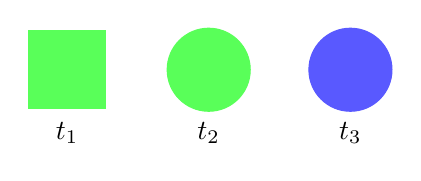
\begin{tikzpicture}
     \path (-1.8, 0) node [shape=rectangle, draw=green!65 ,fill= green!65 ,minimum size=28]{}
           ( 0, 0) node  [shape=circle, draw=green!65, fill= green!65,minimum size=30] {}
           ( 1.8, 0) node [shape=circle, draw=blue!65, fill=blue!65  ,minimum size=30] {}
           ( -1.8, -0.8) node {$t_{1}$}
           ( -0.0, -0.8) node {$t_{2}$}
           (  1.8, -0.8) node {$t_{3}$}
     ;
           
  \end{tikzpicture}
}\hspace{5mm} \subfigure[Vocabulary and truth table]{\label{VaTT}
  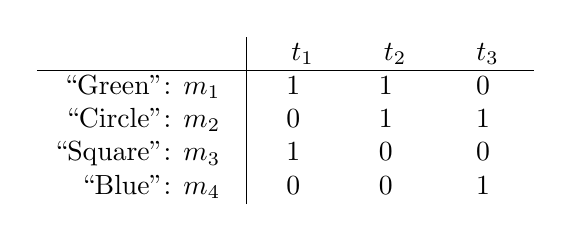
\begin{tikzpicture}
     \path (0,0) node[] 
     {\begin{tabular}{r|ccc}
                         & \quad $t_{1}$\ \  &\quad $t_{2}$\ \  &\quad $t_{3}$ \ \   \\
    \hline
   ``Green'':  $m_{1}$ \quad  &  $1$        &   $1$       & $0$      \\
   ``Circle'': $m_{2}$  \quad &  $0$        &   $1$       & $1$      \\ 
   ``Square'': $m_3$ \quad    &  $1$      &   $0$       & $0$      \\
   ``Blue'':   $m_4$  \quad  &  $0$        &   $0$       & $1$     
     \end{tabular}
     } ;
  \end{tikzpicture}
  }
  \caption{A simple referential game}
\end{figure}


Let us first try to play this game ourselves, to get a better sense of
what it is about and why it is relevant to human pragmatic
reasoning. For simplicity let us assume that the utterances that the
speaker is allowed to use are from a \emph{vocabulary} which is
commonly known between the speaker and the listener. The content of
the vocabulary and the (truth-conditional/literal) meaning of each
word are shown in Figure \ref{VaTT}. Suppose we play as the speaker
and the target is $t_1$, the green square. We can either use
``Square'' or ``Green'' to truthfully refer to it, but it seems more
prudent to use ``Square'', as there is only one square in the context
and thus the listener can easily identify it, whereas there are two
green objects, which makes ``Green'' ambiguous. In terms of the
Gricean \emph{Maxim of Quantity}, we should use ``Square'' because it
is more informative than ``Green'' in the given context; the surplus
informativity moreover seems relevant. Similarly, we should use
``Blue'' to refer to $t_3$, the blue circle. However, using ``Blue''
to refer to the blue circle might intuitively sound a little
unnatural, as color terms are usually used as adjectives\footnote{They
  are used as nouns mostly to refer to the colors themselves.}, while
we usually use nouns to refer to concrete objects. This inclination
becomes more evident when we want to refer to $t_2$, the green
circle. While ``Green'' and ``Circle'' are equally ambiguous in this
case, we might nevertheless prefer the latter.

Now let us turn to play as the listener. If we hear ``Square'' or
``Blue'', we easily know the intended referent as there is no
ambiguity, but what if we hear ``Circle'' (or ``Green'')? There are
two circles in the context that we need to choose from. On the one
hand, the blue circle, having the unique color in the context, seems
to be perceptually dominant and thus easily captures our attention. On
the other hand, from the previous analysis we know that if the blue
circle were the intended referent, the speaker could have chosen
``Blue'' which is not ambiguous and thus more informative. Hence the
listener needs to balance two sources of information, i.e., the
(presumably subconscious) perceptual salience of different objects and
the rational expectation of the likelihood of the speaker making the
utterance for each object. The latter line of reasoning is crucial to
the classic Gricean account of scalar implicatures, and the major
challenges in terms of formal modeling are how to quantify notions
such as informativeness and how different pieces of information should
be integrated.

The RSA model addresses the problems by using information-theoretic
concepts to measure informativeness and Bayesian inference to
integrate different sources of information
\cite{Frank2009,Frank,Bergen2012,GoodmanStuhlmuller2013:Knowledge-and-I}. In
order to measure the informativeness of an utterance, the RSA model
starts with the literal listener who upon receiving an utterance $m$
does a conditioning on its literal meaning:
\begin{equation}\label{Bayesian_literal}
\rho_0(t \mid m) = \mathcal{U}(t\mid \intp{m}) ,
\end{equation}
where $\mathcal{U}$ is a uniform distribution over all the possible
referents. The informativeness of utterance $m$ for the intended
referent $t$ can be measured as the negative Kullback-Leibler
divergence of the induced literal listener's belief $\rho_0$ from the
speaker's own belief $\delta_t$:
\begin{equation} \label{Bayesian_sender_informativeness}
\mbox{Info}(m,t)=-\mbox{KL}(\delta_t \| \rho_0)=-\sum_{t'}\delta_t(t')\log\left(\frac{\delta_t(t')}{\rho_0(t')}\right),
\end{equation}
where $\delta_t$ is a delta distribution with all probability mass on
target object $t$, as the speaker knows her intended referent:
\begin{equation} \label{Bayesian_sender_delta}
\delta_t(t')=\left\{ \begin{array}{ll}
1 & \mbox{if } t' = t \\
0 & \mbox{otherwise}
\end{array}\right. \enspace .
\end{equation}

The speaker acts sub-optimally by choosing the utterance that soft-maximizes her expected utility, which is defined as the informativeness of the utterance subtracted by its cost:
\begin{equation} \label{Bayesian_sender_softmax}
\sigma(m \mid t) \propto \exp(\lambda_\mathrm{S}\cdot \mbox{U}(m,t))=\exp(\lambda_\mathrm{S} \cdot (\mbox{Info}(m,t)-\mbox{Cost}(m))),
\end{equation}
where $\lambda_\mathrm{S}$ is a parameter measuring the speaker's
degree of rationality, i.e., to what extent the speaker sticks to the
strict optimum. The cost term is used to encode preference in
different utterances, be it about the utterances' lengths or syntactic
categories.

From (\ref{Bayesian_literal})-(\ref{Bayesian_sender_softmax}) we obtain the speaker's production rule:

\begin{equation} \label{Bayesian_speaker}
\sigma(m \mid t) \propto \exp(\lambda_\mathrm{S} \cdot (\log \mathcal{U}(t\mid \intp{m})-\mbox{Cost}(m))) \enspace .
\end{equation}

The pragmatic listener in the RSA model, upon receiving the utterance
$m$, performs a Bayesian update on his prior belief $\mathcal{S}(t)$
by using an estimate of the speaker's behavior
(\ref{Bayesian_speaker}):
\begin{equation} \label{Bayesian_rec_update}
\rho(t \mid m) \propto \mathcal{S}(t)\cdot \sigma(m \mid t) \enspace .  
\end{equation}
Bayes' rule naturally integrates the perceptual salience of each
object, which is treated as the prior $\mathcal{S}(t)$ and can be
empirically measured, with listener's expectation of the speaker being
informative, which is incorporated as the likelihood, thus addressing
the previously mentioned challenge of balancing different sources of
information. Setting $\lambda=1$ and $\mbox{Cost}(m)=0$ for all $m$,
\cite{Frank} obtained a highly significant correlation between the
model prediction and their experiment data on actual speaker and
listener behavior gathered from referential games of varying
complexity.


%%% Local Variables: 
%%% mode: latex
%%% TeX-master: "main"
%%% TeX-PDF-mode: t
%%% End:
%%%%%%%%%%%%%%%%%%%%%%%%%%%%%%%%%%%%%%%%%%%%%%%%%%


%%%%%%%%%%%%%%%%%%%%%%%%%%%%%%%%%%%%%%%%%%%%%%%%%%
\section{Alternatives in Design Choices}
\label{sec:alternatives}

The RSA model has a theoretical advantage over traditional formal
pragmatic theories in that it provides quantitative predictions, and
it has been shown to fit relevant empirical data well. However, if we
want to learn more about pragmatic reasoning about referential
expressions, it will be worthwhile to examine RSA carefully to pin
down its major components, to spell out its main design choices and
their underlying assumptions, and to test their contribution to the
predictive power of the model through statistical comparison with
natural alternatives. In this section, we will therefore compare the
RSA model to closely related game theoretic approaches, that likewise
assume that speakers and listeners form cascading beliefs about mutual behavior
and seek to optimize their behavior based on these beliefs
\cite{Rabin1990:Communication-b,Stalnaker:SayingMeaningCredibility,BenzvanRooijOptimalAssertions2007,Franke2011:Quantity-Implic,Jager2013:Rationalizable-}.\footnote{See
\cite{FrankeJager2013:Pragmatic-Back-} for overview and comparison
of game theoretic and Bayesian models.} We will describe a class of potential 
alternatives to RSA and then compare the predictive power of these alternatives 
on relevant empirical data in later sections.

There are three closely related notions, i.e., \emph{belief},
\emph{goal} and \emph{action}, that play a crucial role in RSA as well
as game theoretic models. The relation and distinction between them
can be best illustrated by looking at (\ref{Bayesian_speaker}),
repeated here:
$$\sigma(m \mid t) \propto \exp(\lambda_\mathrm{S} \cdot (\log \mathcal{U}(t\mid \intp{m})-\mbox{Cost}(m))) \enspace .$$
The term $\mathcal{U}(t\mid \intp{m})$ is the speaker's \emph{belief}
about the listener's interpretation of the utterance. The expected
utility $\mbox{U}(m,t)=\log \mathcal{U}(t\mid
\intp{m})-\mbox{Cost}(m)$ describes the speaker's \emph{goal} of
communication, i.e., inducing a belief that is as close as possible to
her own with minimal effort. The production rule $\sigma(m \mid t)$ on
the left-hand side specifies the speaker's \emph{action}, as it
defines the probability with which, according to RSA, speakers would
choose a particular expression. The soft-max rule connects these
notions, as a (sub-)rational agent's action depends on his belief and
goal. While the RSA and game theoretic models all share this general
architecture in their designs, they vary in the specific
interpretations of the three ingredients, which reflect different
views and emphasis on language and communication and give rise to a
series of interesting and important empirical questions. Again, let us
continue with the speaker model (\ref{Bayesian_speaker}) to illustrate
some points of divergence and formally define the corresponding
alternatives.

First of all, although it is prima facie reasonable to hypothesize, as
\cite{Frank} do, that the empirically measured perceptual salience
$\mathcal{S}(\cdot)$ is common knowledge between speaker and listener,
it does not actually affect RSA's production rule
(\ref{Bayesian_speaker}) at all. This makes it unclear in what sense
the speaker can be said to know the listener's perceptual salience,
since neither his beliefs nor actions depend on it. A natural variant,
which is used in some game theoretic models, would be to replace the literal
listener's uniform distribution $\mathcal{U}(t)$ in
(\ref{Bayesian_literal}) with the salience prior
$\mathcal{S}(t)$. This leads to the alternative production rule:
\begin{equation} \label{Bayesian_speaker_salience}
\sigma_\mathcal{S}(m \mid t) \propto \exp(\lambda_\mathrm{S} \cdot (\log \mathcal{S}(t\mid \intp{m})-\mbox{Cost}(m))) \enspace .
\end{equation}


Secondly, RSA measures the informativeness of an utterance $m$, which
is a crucial part of the communicative goal, in terms of how close the
induced belief of the literal listener is from the speaker's own
belief. This means that the RSA model sees the goal of communication
as conveying belief. While it is normally true that language does
convey the belief of the speaker, it is questionable at least in this
referential scenario whether letting the listener form a proper belief
is the ultimate goal of the communication. After all, if the speaker
wants to refer to something, it seems that in the end what matters is
whether the listener actually picks out the intended referent
successfully (e.g., when the speaker wants the listener to pass
something). This view is inherent in game theoretic approaches where
agents' beliefs are backed up by explicit formulations of their
utilities. We might call this latter view \emph{action-oriented}, in
contrast to the \emph{belief-oriented} view of communication which the
RSA model adopts, as it interprets the goal of communication as
invoking the intended action rather than forming an accurate
belief.\footnote{Note that the two views are clearly intimately
  related, despite our emphasis on their differences here. An accurate
  belief is usually helpful for choosing a desired action. In fact,
  forming a belief can itself be seen as an action that the listener
  performs, which might well be all that the speaker cares about in
  many everyday situations, e.g., casual talks or responses to
  inquiries of information. Also, the relevant actions might vary
  greatly across situations which makes belief formation a practical
  alternative to serve as the goal. Nevertheless, they are still
  essentially different views in spite of the fact that they often
  coincide in practice. The referential communication scenario we
  investigate in this paper reflects the distinction.} Thus, according
to this view, the informativeness of a message would be measured as
the probability of the listener choosing the intended
referent. Formally speaking, we have the action-oriented speaker model\footnote{There might be concern about whether there should be another soft-max step for the literal listener's choice probability $\rho_0(t\mid m)$ in order for it to be action-oriented. 
This depends on the precise conceptual status of the literal listener in the model and to our knowledge there is no consensus yet. We tend to think of a literal listener as an automatic subconscious process that involves no optimality reasoning or decision-making. Thus we consider it appropriate to use $\rho_0(t\mid m)$ as the action of the literal listener. However, we do agree that in principle there can be a model whose literal listener does a soft-max over the salience prior, and such a model can be similarly included in the model comparison.}:
  
\begin{equation} \label{Bayesian_speaker_action}
\sigma_\mathrm{a}(m \mid t) \propto \exp(\lambda_\mathrm{S} \cdot (\rho_0(t\mid m)-\mbox{Cost}(m))) \enspace .
\end{equation}

Hence we have four types of speaker models that differ in either the speaker's belief about the literal listener, or the speaker's goal of communication. We now introduce a uniform notation $\sigma_{xy},\ x\in\{\mathrm{a},\mathrm{b}\},y\in\{\mathcal{U},\mathcal{S}\}$ for them:
\begin{equation} \label{Bayesian_speaker_uniform_action}
\sigma_{\mathrm{a}y}(m \mid t) \propto \exp(\lambda_\mathrm{S} \cdot ( y(t\mid m)-\mbox{Cost}(m))),
\end{equation}
\begin{equation} \label{Bayesian_speaker_uniform_belief}
\sigma_{\mathrm{b}y}(m \mid t) \propto \exp(\lambda_\mathrm{S} \cdot (\log y(t\mid m)-\mbox{Cost}(m))),
\end{equation}
where $\mathcal{U}$ is the uniform prior and $\mathcal{S}$ is the
salience prior. For example, in the original RSA model, the speaker
does not take listener's salience prior into account and he has a
belief-oriented goal of communication. Thus it will be denoted as
$\sigma_{\mathrm{b}\mathcal{U}}$.

Finally, the original RSA speaker model of \cite{Frank} has
$\mbox{Cost}(m)=0$ for all $m$, which means that the potential speaker
preference in different utterances is not taken into account (but not
so in, e.g., \cite{Bergen2012}). As we previously pointed out, our
intuition seems to suggest a preference for nouns over adjectives as
referential expressions.\footnote{The rich tradition on referential
  expression generation \cite{KramerDeemter2012:Computational-G} has
  also identified the need to take speaker preferences into account,
  and \cite{GattGompel2013:Are-we-Bayesian} criticize RSA on these
  grounds as well.} Since it is an empirical question whether, to what
direction or to what extent such a preference exists, we leave open
all the possibilities. Technically speaking, since only the difference
in costs matters, we define the cost function using a constant $c\in
\mathbb{R}$
\begin{equation} \label{cost}
\mbox{Cost}(m)=c \mbox{ if } m \mbox{ is an adjective and }0 \mbox{ otherwise} \enspace . 
\end{equation}
If $c>0$ it means there is a preference for nouns and if $c<0$ then the preference is for adjectives. No preference exists if $c=0$.

Now we turn to the listener model (\ref{Bayesian_rec_update}), where the boundary between belief, goal and action becomes less clear:
$$\rho(t \mid m) \propto \mathcal{S}(t)\cdot \sigma(m \mid t) \enspace . $$

Let us start from the relatively clear part. As pointed out
previously, the likelihood term $\sigma(m \mid t)$ is the listener's
belief about how the speaker behaves. One natural question is to what
extent the listener's belief correlates with the actual production. We
thus treat the speaker's production term $\sigma(m \mid t)$ in the
listener's model as a parameter, making the association with a belief
about production of the listener model explicit:
\begin{equation} \label{listener-production}
\rho(\sigma_{xy})(t \mid m) \propto \mathcal{S}(t)\cdot \sigma_{xy}(m \mid t) \enspace .
\end{equation}
Note that the speaker's production rule has two parameters
$\lambda_\mathrm{S},c$ which are also included in the above
specification of the listener model.

Next, even though our intuition suggests different objects have different perceptual salience and thus might affect our judgment, it is after all an empirical question whether it is relevant in the interpretation of referential expressions. It is in principle possible that the listener does not take into account the perceptual salience in his reasoning, which means he has a uniform prior over the referents:
\begin{equation} \label{listener-production-uniform}
\rho_{\mathcal{U}}(\sigma_{xy})(t \mid m) \propto \mathcal{U}(t)\cdot \sigma_{xy}(m \mid t) \enspace .
\end{equation}

Finally, since the RSA model adopts a belief-oriented view on the goal
of communication, its listener model only consists of the belief about
the intended referent after hearing the utterance, obtained by a Bayes
update. However, according to the action-oriented view, this is not
quite the end of the story. The listener often needs to decide the
exact referent of a referential expression. (Again, consider the case
in which the listener is asked to pass something.) Hence in such cases
the listener will choose an object by, essentially, (soft-)maximizing
over his beliefs. Formally, the action-oriented listener model
becomes:
\begin{equation} \label{listener-action}
\rho_{\mathrm{a}v}(\sigma_{xy})(t \mid m) \propto \exp(\lambda_\mathrm{L} \cdot \rho_{\mathrm{b}v}(\sigma_{xy})(t \mid m) ),
\end{equation}
where $v\in\{\mathcal{U},\mathcal{S}\}$, $\lambda_\mathrm{L}$ is the
parameter measuring the listener's degree of rationality, and
$\rho_{\mathrm{b}v}$ is the belief-oriented model that does the
Bayesian update:
\begin{equation} \label{listener-belief}
\rho_{\mathrm{b}v}(\sigma_{xy})(t \mid m) \propto v(t)\cdot \sigma_{xy}(m \mid t) \enspace .
\end{equation}
For instance, the original RSA listener model is a belief-oriented one with the perceptual salience as prior, whose belief about the speaker is $\sigma_{\mathrm{b}\mathcal{U}}$, hence it is denoted as $\rho_{\mathrm{b}\mathcal{S}}(\sigma_{\mathrm{b}\mathcal{U}})$.


%%% Local Variables: 
%%% mode: latex
%%% TeX-master: "main"
%%% TeX-PDF-mode: t
%%% End:
%%%%%%%%%%%%%%%%%%%%%%%%%%%%%%%%%%%%%%%%%%%%%%%%%%


%%%%%%%%%%%%%%%%%%%%%%%%%%%%%%%%%%%%%%%%%%%%%%%%%%
\section{The Experiment}
\label{sec:experiment}

In the previous section we analyzed the design of the original RSA model, spelled out the relation and distinction between belief, goal and action, and proposed a familiy of alternative models based on different interpretation of these notions. This gives rise to a series of interesting empirical questions regarding the underlying assumptions of the models. In order to gain insight into these questions by comparing the predictive power of different models, we conducted the following experiment to collect empirical data, which we will use to test the predictions of different models in the next section.

\subsection*{Participants}

We recruited 1032 US Participants via Amazon Mechanical Turk, an online crowd-sourcing tool. Each participant played a one-shot referential game either as a speaker or as a listener and received a payment of 5 cents. If a participant contributed multiple trials, only the first was included. All participants passed the attention check described below.

\subsection*{Materials and Procedure}

Each participant saw a context consisting of three objects (Figure \ref{exp_context} as an example) and reported on the number of objects in the context as an attention check. Participants in the listener conditions were told to imagine someone was talking to them and used some utterance (depending on the exact condition) to refer to exactly one of the objects in the context. Then they were asked to choose what they thought to be the intended referent. Participants in the speaker conditions were told to imagine they were talking to someone and they wanted to refer to one of the objects (indicated by a small red arrow\footnote{Participants were told that the arrow was only for illustration and thus the person they were talking to could not see it.}). Then they were asked to choose between two words to refer to it. 

\begin{figure}[htb] 
  \centering
  
\begin{tikzpicture}
     \path (-1.4, 0) node [shape=rectangle, draw=green!65 ,fill= green!65 ,minimum size=28]{}
           ( 0, 0) node  [shape=circle, draw=green!65, fill= green!65,minimum size=30] {}
           ( 1.4, 0) node [shape=circle, draw=blue!65, fill=blue!65  ,minimum size=30] {}
     ;
           
  \end{tikzpicture}
  
  \caption{A sample context}\label{exp_context}
\end{figure}

Each context had a square and a circle sharing the same color, and another circle having a different color. Hence each object had two features: shape (square/circle) and color (green/blue) and each context had two ambiguous (shared by two objects) features. In the listener salience condition, participants were told that the person talking to them was using a foreign language they could not understand, and in the other two listener conditions, the utterances used were the ambiguous feature of shape and color, respectively. In the speaker conditions, the target could be any of the three objects: the one with the unique color, the one with the unique shape and the one with both features shared. The two words for the participants to choose between were the features of color and shape of the target object.

The positions and colors of the objects, as well as the orders of the candidate words in the speaker conditions, were counterbalanced. 

\subsection*{Design}

There are four major designs in our own experiment that differ from the original experiment in \cite{Frank}. First of all, the original experiment used the betting paradigm, i.e. participants were asked to bet over a range of options and they were instructed that the amount of money that is bet on an option should reflect their confidence that the option is correct. Even though the betting paradigm has the merit of providing us with graded reponses from each individual participant, the caveat is that it is unclear whether it measures the belief or the action. This can lead to confusion when we are to fit the model predictions to the empirical data without knowing whether they are directly comparable. In addition, since the betting paradigm is more or less introspective in nature, it tends to be not very accurate. Thus we used forced choice in our experiment instead, which clearly measures the action and does not rely on introspection.
Secondly, since we decided to investigate the influence of the speaker's preference as well as the listener's perceptual salience, we focused on contexts equivalent to Figure \ref{context}, which are most typical in Gricean accounts of scalar implicature, and examined different features separately.
Thirdly, we only included the features of color and shape to ensure the vocabulary to be common knowledge, excluding the feature of texture. Finally, we did not use dotted line surrounding an object as the way to indicate the target to the speaker, as it could emphasize the feature of shape and thus add confound in the experiment. Instead we used a small arrow pointing to the target. 

Despite these differences, the remaining aspects in our experiment were almost identical to those of the original one, e.g. the phrasing of the instructions.

\ 

The results of the speaker and listener conditions of our experiment are shown as follows.

 
\subsection{Speaker Conditions}

There were 432 participants in the speaker conditions, 144 in each condition. The numbers of participants choosing each word in each condition are shown in Table \ref{table:speaker}. Note that when the target was the object with the unique shape (as in the first row of the table), the feature of shape (``Square'' in the example) should be the optimal utterance because the listener could uniquely identify it. Similarly when the target was the object with the unique color (the second row), the optimal utterance would be the feature of color (``Blue''). When the target was the object with both features shared, both features should be equally ambiguous because of the context's symmetric nature.

\begin{table}[htb]   
  \caption{Speaker Conditions}
  \centering
  \begin{tabular}{c|ccccc}
   Target  & ``Green'' & ``Square'' & ``Blue'' & ``Circle'' & Total\\ 
     \hline
\textcolor{green!65}{\Large{$\blacksquare$}}    & $9$        &   $135$   & -- & -- &144\\
\textcolor{blue!65}{\Huge{$\bullet$}}           & --        &   --      & $119$ & $25$ & 144\\
\textcolor{green!65}{\Huge{$\bullet$}}          & $63$        &   --    &  --   & $81$             &144
  \end{tabular}

  \label{table:speaker}
\end{table}

From the data in Table \ref{table:speaker}, we can see that the speakers tend to choose the optimal feature more often when the target has the unique shape than when it has the unique color ($\chi^2=8.5, p<.01$). Even though they seem to prefer the feature of shape when the target's both features are shared, the difference is not statistically significant from uniform random choice ($\chi^2=2.25, p=.13$).


\subsection{Listener Conditions}

There were 600 participants in the listener conditions, 240 in the salience condition and 180 in each of the remaining two conditions. The numbers of participants choosing each object in each condition are shown in Table \ref{table:listener}. 

\begin{table}[htb] 
  \caption{Listener Conditions}
  \centering
\begin{tabular}{c|cccc}
   & \quad \textcolor{green!65}{\Large{$\blacksquare$}}&  \textcolor{green!65}{\Huge{$\bullet$}}& \textcolor{blue!65}{\Huge{$\bullet$}} & Total\\ 
     \hline
 Salience   \quad  & \quad  $71$      \quad    &   $30$    \quad     & $139$ \quad     & $240$      \\
 ``Green''   \quad  & \quad  $65$      \quad    &   $115$    \quad     & $0$ \quad     & $180$     \\
 ``Circle''   &  \quad $1$        &    $62$        & $117$ \quad     & $180$
  \end{tabular}

  \label{table:listener}
\end{table}

The result of the salience condition will be used as the empirical estimation of contextual salience. For the other two conditions, the object with both features shared (the green circle in the above table, but note that we counterbalanced colors) is what the Gricean pragmatic account predicts to be the target. The result in Table \ref{table:listener} shows that when the message is ``Green'', listeners prefer the green circle which is predicted by the Gricean pragmatics, while they tend to stick to the blue circle which is more perceptually salient when the message is ``Circle''. The behavioral patterns in both conditions are significantly different from uniform random choice, and they significantly differ from each other in respect of whether they conform to the predictions by Gricean pragmatic theory.


%%%%%%%%%%%%%%%%%%%%%%%%%%%%%%%%%%%%%%%%%%%%%%%%%%


%%%%%%%%%%%%%%%%%%%%%%%%%%%%%%%%%%%%%%%%%%%%%%%%%%
\section{Model Comparison}
\label{sec:model-comparison}

We use a Bayesian approach to model comparison to find out which model
best explains the data described in the previous section
\cite{VandekerckhoveMatzke2013:Model-Compariso}. The models under
investigation have unspecified parameters: the speaker's degree of of
rationality $\lambda_\mathrm{S}$, the cost of adjectives $c$, and, for
those listener models that have an action-oriented communication goal
, the listener's degree of rationality $\lambda_\mathrm{L}$. Since
there is no principled theory to determine the value of the
parameters, we will rely on relatively uninformed hyperpriors
(so-called to distinguish them from the salience priors). Based on a
specification of hyperpriors, we calculate the models' \emph{evidence}
and compare them by their \emph{Bayes factors}. The evidence of a
model $M$ is the weighted average of the likelihood of observing the
data under all parameter values:
\begin{align}
  \label{BMA}
  \mathrm{Ev}(M)= \int \Pr(\theta) \cdot p(D | M, \theta)\, \mathrm{d}\theta,
\end{align}
where $\Pr(\theta)$ is the hyperprior over parameter(-tuple) $\theta$
associated with $M$ and $D$ is the observed data. The Bayes factor
$K^{M_1}_{M_2}$ is a comparative measure for the plausibility of model
$M_1$ over $M_2$, given their respective hyperpriors and the data in
question:
\begin{align}
  K^{M_1}_{M_2} = \frac{\mathrm{Ev}(M_1)}{\mathrm{Ev}(M_2)} \enspace .
\end{align}
Model $M_1$ makes the data more likely whenever $K^{M_1}_{M_2}$, but
normally only a Bayes factor $K^{M_1}_{M_2} >3$ (or sometimes
$K^{M_1}_{M_2} > 5$) is considered substantial. Values $K^{M_1}_{M_2}
> 10$ are considered strong evidence.

In a sense, comparison by Bayes factors is comparing models in a wider
sense of the term: we actually compare pairs consisting of a model and
its associated hyperprior. For clarity, we refer henceforth to a
model-hyperprior pair as a Model.

\paragraph{Speaker data.} First we look at the speaker models $\sigma_{xy},\
x\in\{a,b\},y\in\{\mathcal{U},\mathcal{S}\}$. Each model has two
parameters $\lambda_\mathrm{S}$ and $c$. We assume that they are
independent of each other:
\begin{equation}\label{hyper-speaker-independent}
\Pr(\lambda_\mathrm{S},c)=\Pr(\lambda_\mathrm{S}) \cdot \Pr(c) \enspace .
\end{equation}
We are uncertain about the rationality of the speaker:
\begin{equation}\label{hyper-speaker-lambda}
\Pr(\lambda_\mathrm{S})= \mathcal{U}_{(0,11)}(\lambda_\mathrm{S}),
\end{equation}
which is a uniform distribution over $(0,11)$. Excluding
$\lambda$-values $\ge 11$ serves practical purposes only, but is
innocuous since the regions of maximum a posteriori likelihood of
$\lambda$ lies safely in the chosen interval for all models. Next, to
allow for the possibility of speaker preferences (nouns over
adjectives or vice versa), we consider two types of hyperpriors for
costs $c$. The first hyperprior has $\Pr(c)= \delta(c)$, the Dirac
delta distribution, that assigns all probability mass $1$ to
$c=0$. This captures the assumption that there is no speaker
preference. The second hyperprior is $\mathcal{U}_{(-0.4,0.4)}$, which
captures the notion that a preference exists, without commitment to
either direction. We restrict our attention to the interval
$(-0.4,0.4)$, because we consider higher levels of cost implausible,
given that utilities for successful communication live in $[0,1]$ and
that we believe that strive for communicative success should outrank
preference satisfaction in a rational model of communication. Taken
together, there are four speaker models, two hyperpriors for each, so
that we compare eight Models with respect to their evidences.

Evidences of speaker Models were calculated by grid approximation. The
results are shown in Table \ref{table:speaker mod}. We can see
\todo{include Hinton diagrams?} that the data very strongly supports
speaker models that do not take the listener's perceptual salience
into account. Also, it seems that action-oriented models are slightly
better than their belief-oriented counterparts, even though the
relevant Bayes factors are not substantial by common
standards. Finally, our data makes each speaker Model that does allow
for a speaker preference strongly more plausible than its
counterpart that does not. A look at the posterior likelihood of $c$
for each speaker model informs us that our data supports the belief
that the speakers have a preference for nouns, see
Figure~\ref{fig:cost_post_s}. \todo{improve plot}
%
\begin{table}[htb] 
  \centering 
  \caption{Evidences of speaker Models}
  \begin{tabular}{lcccc}
    support of $P(c)$ 
    & $\sigma_{\mathrm{b}\mathcal{U}}$
    & $\sigma_{\mathrm{a}\mathcal{U}}$
    & $\sigma_{\mathrm{b}\mathcal{S}}$
    & $\sigma_{\mathrm{a}\mathcal{S}}$
    \\ \midrule
    $[0,0]$
    & 4.93e-30
    & 3.56e-30
    & 5.92e-46
    & 3.09e-69
    \\
    $(-0.4,0.4)$
    & 5.04e-15
    & 4.02e-15
    & 4.28e-36
    & 3.27e-61
  \end{tabular} 
  \label{table:speaker mod}
\end{table}
%
\begin{figure}[htb]
  \centering
  \caption{Posterior distributions over costs given the data for each
    speaker model.}
  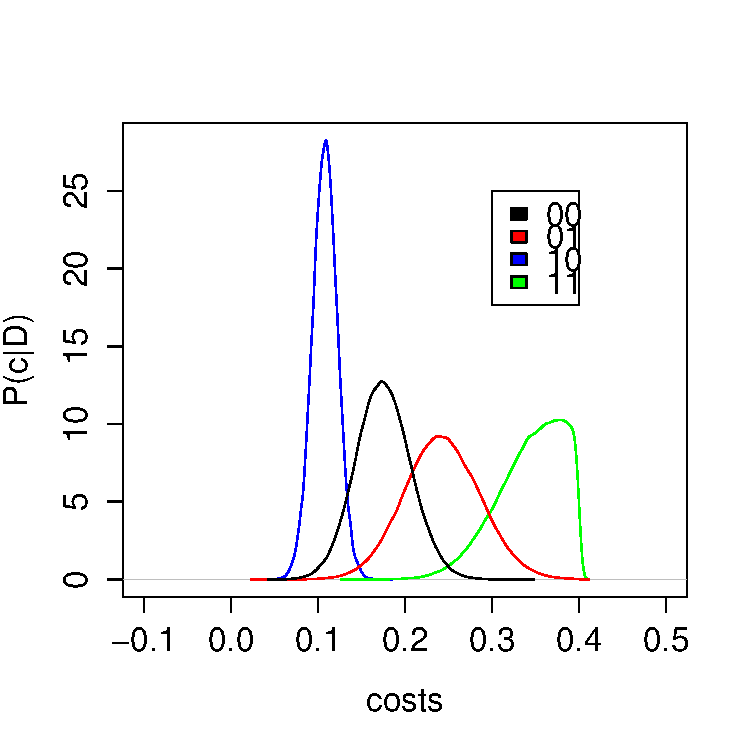
\includegraphics[width=0.5\textwidth]{pics/cost_post_s.pdf}
  \label{fig:cost_post_s}
\end{figure}
%
In sum, our data supports the belief that the speaker does not take
into account the preceptual salience of the listener, while having her
own preference for shape terms over color terms.


\paragraph{Listener data.} Each listener models has a speaker model
nested inside as a belief of the listener about the speaker's
behavior. Section~XYZ \todo{cross-reference} introduced a total of 16
potentially relevant listener models, but we will focus on a selection
only. For one, we restrict our attention to those listener models that
are either entirely belief-based or entirely action-based. In other
words, we exclude models like
$\rho_{\mathrm{a}\cdot}(\sigma_{\mathrm{b}\cdot})$ where the receiver
part assumes an action-based goal structure and the speaker part a
belief-based goal structure. For another, we assume that the
listener's model of the speaker is a reasonable one and therefore put
to the side listener models that have speaker models that are highly
implausible, given the speaker data as discussed above. Effectively,
this discards listener models that include a speaker models that take
the listener's salience prior into account. These two principled
restrictions leave us with four listener models to compare.

Further variation comes from different relevant
hyperpriors. Belief-based models of the listener have the same
parameters as speaker models: the speaker's rationality
$\lambda_\mathrm{S}$ and the speaker's preference costs
$c$. Importantly though, hyperpriors over $\lambda_\mathrm{S}$ and
$c$, although formally parallel to those for speaker models, have a
different interpretation in listener models where they capture our
prior beliefs about the listeners' beliefs about the speakers' likely
rationality and preferences. This is true as well for action-based
models, which also have an additional parameter
$\lambda_\mathrm{L}$. Hyperpriors for the latter encode our prior
beliefs about the listener's actual rationality.

We consider a variety of hyperpriors that differ with respect to
whether they take the speaker's costs into account, whether the
listener's beliefs about the speaker's rationality and preferences are
uninformed (i.e., flat) or informed (i.e., given by the posterior
likelihood of parameters given the actual speaker data) and, in
action-based models, whether the listener's level of rationality
corresponds to his ``informed'' beliefs. The latter option effectively
implements the assumption that there is a tight correlation between
the speaker's actual rationality, the listener's actual rationality
and the listener's beliefs about the speaker's rationality.

Concretely, we call ``flat w/o costs'' the hyperpriors:
\begin{align*}
  \Pr(\lambda_\mathrm{S},c) & =
  \mathcal{U}_{(0,11)}(\lambda_\mathrm{S}) \cdot
  \delta(c) \\
  \Pr(\lambda_\mathrm{S},c,\lambda_\mathrm{L}) & = 
  \mathcal{U}_{(0,11)}(\lambda_\mathrm{S}) \cdot
    \delta(c) \cdot  \mathcal{U}_{(0,11)}(
    \lambda_\mathrm{L}),
\end{align*}
for belief-based and action-based models respectively. Hyperpriors
``flat with costs'' take a wider range of speaker preferences into
account: 
\begin{align*}
  \Pr(\lambda_\mathrm{S},c) & =
  \mathcal{U}_{(0,11)}(\lambda_\mathrm{S}) \cdot
  \mathcal{U}_{(-0.4,0.4)}(c) \\
  \Pr(\lambda_\mathrm{S},c,\lambda_\mathrm{L}) & = 
  \mathcal{U}_{(0,11)}(\lambda_\mathrm{S}) \cdot
    \mathcal{U}_{(-0.4,0.4)}(c) \cdot  \mathcal{U}_{(0,11)}(
    \lambda_\mathrm{L}) \enspace .
\end{align*}

Hyperpriors that capture the idea that the listener's beliefs are good
guesses of speaker behavior are modeled as if informed by the data
from the speaker experiments:
\begin{align*}
  \Pr(\lambda_\mathrm{S},c) & = \Pr(\lambda_\mathrm{S},c \mid D_\mathrm{S}, M_\mathrm{S}) \\
  \Pr(\lambda_\mathrm{S},c,\lambda_\mathrm{L}) & = 
   \Pr(\lambda_\mathrm{S},c \mid D_\mathrm{S}, M_\mathrm{S}) \cdot  \mathcal{U}_{(0,11)}(
    \lambda_\mathrm{L}) \enspace .
\end{align*}
Here, $D_\mathrm{S}$ is the data from the speaker experiments, and
$M_\mathrm{S}$ the relevant speaker model. For a given listener model,
we consider only the embedded speaker model as relevant. We call
hyperpriors of the above form ``informed'' or, in the case of
action-based models, ``informed uncorrelated''. We distinguish the
latter from ``informed correlated'' hyperpriors of the form:
\begin{align*}
  \Pr(\lambda_\mathrm{S},c,\lambda_\mathrm{L}) & = 
   \Pr(\lambda_\mathrm{S},c \mid D_\mathrm{S}, M_\mathrm{S}) \cdot \Pr(\lambda_\mathrm{L} \mid D_\mathrm{S}, M_\mathrm{S}),
\end{align*}
where the listener's rationality parameter is distributed according to
the relevant posterior (marginalized over costs). All of the three
types of informed hyperpriors were tested in two varieties: whether
the listener takes the sender's preferences into account or not. If he
does not, the posterior $\Pr(\lambda_\mathrm{S},c \mid D_\mathrm{S},
M_\mathrm{S})$ is derived from a speaker-hyperprior $\Pr(c) =
\delta{c}$; otherwise from $\Pr(c) = \mathcal{U}_{(-0.4,0.4)}(c)$.

Taken together, we consider two belief-based models, paired with four
hyperpriors, and two action-based models, paired with six hyperpriors
(see Table~XYZ\todo{reference}). Comparing these ten Models is meant
to address the following general questions:
\begin{enumerate}
\item Is the goal structure assumed by participants in our task
  belief-based or action-based?
\item Does the listener take the estimated salience prior into account
  or not?
\item Is the listener's belief in the speaker's level of rationality
  ``correct'', i.e., in line with the observed speaker data?
\item Is the listener's level of rationality related to the speaker's
  actual level of rationality?
\end{enumerate}




\begin{table}[htb]
  \centering
  \caption{asdf}
  \begin{tabular}{llr}
    belief-based 
    & action-based
    & 
    \\
    $\Pr(\lambda_\mathrm{S},c)$
    & $\Pr(\lambda_\mathrm{S},c,\lambda_\mathrm{L})$
    & label
    \\ \midrule
    $\mathcal{U}_{(0,11)}(\lambda_\mathrm{S}) \cdot \mathcal{U}_{[0,0]}(c)$
    & $\mathcal{U}_{(0,11)}(\lambda_\mathrm{S}) \cdot
    \mathcal{U}_{[0,0]}(c) \cdot  \mathcal{U}_{(0,11)}(
    \lambda_\mathrm{L})$
    & flat, w/o costs
    \\
    $\mathcal{U}_{(0,11)}(\lambda_\mathrm{S}) \cdot \mathcal{U}_{(-0.4,0.4)}(c)$
    & $\mathcal{U}_{(0,11)}(\lambda_\mathrm{S}) \cdot
    \mathcal{U}_{(-0.4,0.4)}(c) \cdot  \mathcal{U}_{(0,11)}(
    \lambda_\mathrm{L})$
    & flat, with costs
    \\
    $\Pr(\lambda_\mathrm{S},c \mid D_\mathrm{S}, M_\mathrm{S})$
    & $\Pr(\lambda_\mathrm{S},c \mid D_\mathrm{S}, M_\mathrm{S}) \cdot  \mathcal{U}_{(0,11)}(
    \lambda_\mathrm{L})$
    & informed uncorrelated, w/o costs
    \\
    $\mathcal{U}_{(0,11)}(\lambda_\mathrm{S}) \cdot \mathcal{U}_{(-0.4,0.4)}(c)$
    & $\mathcal{U}_{(0,11)}(\lambda_\mathrm{S}) \cdot
    \mathcal{U}_{(-0.4,0.4)}(c) \cdot  \mathcal{U}_{(0,11)}(
    \lambda_\mathrm{L})$
    & informed uncorrelated, with costs
    \\
  \end{tabular}
  \label{tab:hyperpriors_l}
\end{table}


\vspace{1cm}
\hrule
\vspace{1cm}



 Since we want to know how such a belief correlates with the
actual production, we put two kinds of hyperpriors under
investigation. On the one hand, the flat-independent hyperpriors treat
different parameters as independent:
\begin{equation}\label{hyper-listener-independent}
\Pr(\lambda_\mathrm{S},c,\lambda_\mathrm{L})=\mathcal{U}_{(0,11)}(\lambda_\mathrm{S}) \cdot \Pr(c) \cdot  \mathcal{U}_{(0,11)}( \lambda_\mathrm{L}) \enspace .
\end{equation}
On the other hand, the true-correlated hyperpriors use the data from the speaker condition to estimate the hyperpriors for $\lambda_\mathrm{S}$ and $c$, and let $\lambda_\mathrm{L}$ have the same distribution as $\lambda_\mathrm{S}$:
\begin{equation}\label{hyper-listener-independent}
\Pr(\lambda_\mathrm{S},c,\lambda_\mathrm{L})=\mathcal{U}_{(0,11)}(\lambda_\mathrm{S} \mid D_\mathrm{S}, M_\mathrm{S}) \,\Pr(c\mid D_\mathrm{S}, M_\mathrm{S})  \,\mathcal{U}_{(0,11)}( \lambda_\mathrm{L} \mid D_\mathrm{S}, M_\mathrm{S}),
\end{equation}
and thus put a stronger constraint on the listener's belief about the speaker. 

The comparison result of the speaker models are shown in Table \ref{table:listener mod}. The best model, which is substantially better than the rest, is action-oriented and takes perceptual salience into account. It has a true-correlated speaker model which is action-oriented and does not take perceptual salience nor speaker preference into account. Note that the nested speaker model is different from the best actual speaker model only in that it does not incorporate speaker preference.  

\begin{table}[htb] 
\caption{Listener Model Comparison}
  \centering 
  \begin{tabular}{ccccc}
    rank
    & model
    & hyperprior
    & sp.~pref.
    & evidence 
    \\ \hline
    1 
    & $\rho_{\mathrm{a}\mathcal{S}}(\sigma_{\mathrm{a}\mathcal{U}})$
    & true correlated
    & $-$
    & 1.11E-003
    \\ \\
    2 
    & $\rho_{\mathrm{ a}\mathcal{S}}(\sigma_{\mathrm{b}\mathcal{U}})$
    & true correlated
    & $-$
    & 2.36E-004
    \\     
    3 
    & $\rho_{\mathrm{b}\mathcal{U}}(\sigma_{\mathrm{b}\mathcal{S}})$
    & flat independent \quad
    & adj.~or nouns \quad
    & 1.29E-004
    \\     
    4 
    & $\rho_{\mathrm{a}\mathcal{U}}(\sigma_{\mathrm{b}\mathcal{S}})$
    & flat independent
    & none
    & 9.94E-005
    \\     
    5 
    & $\rho_{\mathrm{a}\mathcal{U}}(\sigma_{\mathrm{b}\mathcal{S}})$
    & flat independent
    & adj.~or nouns
    & 8.79E-005
    \\
    $\vdots$\\
    14 
    & $\rho_{\mathrm{b}\mathcal{S}}(\sigma_{\mathrm{b}\mathcal{U}})$
    & flat independent
    & adj.~or nouns
    & 5.31E-005
    \\
    $\vdots$\\
    19 
    & $\rho_{\mathrm{b}\mathcal{S}}(\sigma_{\mathrm{b}\mathcal{U}})$
    & true correlated
    & $-$
    & 2.91E-005
    \\
    $\vdots$
  \end{tabular}
  \label{table:listener mod}
\end{table}

Combining the model comparison results for both the speaker and the listener models, it seems that if we treat the speaker's preference as some lexical salience which together with the listener's perceptual salience constitutes the contextual salience of the referential game, then contextual salience actually manifests \emph{lack of} common knowledge between the speaker and the listener rather than the presence of it, since they both have some preference that biases their decisions but they are unaware of each other's such preference. However, there is indeed something common between the speaker and the listener, i.e. the distribution of the degree of rationality. Also, the listener's belief about the speaker is correct modulo the speaker's private lexical salience. 


%%% Local Variables: 
%%% mode: latex
%%% TeX-master: "main"
%%% TeX-PDF-mode: t
%%% End:
%%%%%%%%%%%%%%%%%%%%%%%%%%%%%%%%%%%%%%%%%%%%%%%%%%


%%%%%%%%%%%%%%%%%%%%%%%%%%%%%%%%%%%%%%%%%%%%%%%%%%
\section{Conclusion}
\label{sec:conclusion}

Our experiment and model comparison suggest the following: (1) On the
conceptual level, it is helpful to clarify the distinction between
belief, goal and action, and the Bayesian framework provides us with a
natural way to structure these components into a formal model. By
examining each component systematically, we can explicitly spell out
the underlying assumptions and formulate alternative hypotheses to be
tested. (2) On the empirical level, we tested the RSA model with a
family of variants motivated from a game theoretic perspective on
communication, and in particular, we investigated the speaker's
preference as well as the listener's perceptual salience. Our data
showed a more intricate picture of the roles that various factors play
in pragmatic reasoning about referential expressions. We found
evidence for a correlation between the speaker's and the listener's
rationality. Either side appears to have his own biases, but appears
to be negligent of the other's. Also, an action-based view might
better reflect the goal of communication, at least in the
forced-choice experimental setting. Understanding the relation between
the forced-choice and the betting paradigms would be an important next
step to gain more insight into the differences between action- and
belief-based goal structures.

The set of models we were able to compare explicitly here does clearly
not exhaust the space of plausible candidates. For example, we
excluded listener models in which the literal listener takes the
salience prior into account. As an anonymous reviewer points out, this
may seem paradoxical because the best listener models of our
comparison do assume that the actual pragmatic listener takes salience
into account, but does not believe that the speaker believes that he
does. But actually, there is no friction here at all, because the
listener model that is embedded in a speaker model is a different one
from the full pragmatic listener model. If we think of the pragmatic
listener as simulating his own hypothetical speaker behavior, there is
nothing puzzling about factoring in salience only at a higher level of
pragmatic inference.

A similar issue arises with respect to the rationality parameters in
action-based listener models. We assumed that there are two
rationality parameters, one for the listener's actual rationality and
one for the listener's beliefs about the speaker's rationality. But we
also saw that a model that correlates the set of joint values of these
parameter pairs gave the best predictions of our data. This raises
many interesting issues for further research, most of which we cannot
answer here. The most obvious idea is, of course, to equate the
speaker's and the listener's lambda and so that the listener would
believe that the speaker is exactly as rational as the listener
himself. Surprisingly, this model achieves a very poor fit on our
data, despite its parsimony. More research into correlations in
perspective-taking and beliefs in rationality will hopefully shed more
light on this fascinating issue.

In summary, our work shows that careful conceptual analysis of the
design choices for quantitative models can lead to a better
understanding of the phenomenon and further improvement in the formal
model's predictive power. Of course, our restricted empirical data can
only serve as a start and more data is needed to fuel further model
comparison towards a more robust pragmatic theory of people's
probabilistic reasoning about referential expressions.

%%% Local Variables: 
%%% mode: latex
%%% TeX-master: "main"
%%% TeX-PDF-mode: t
%%% End:
%%%%%%%%%%%%%%%%%%%%%%%%%%%%%%%%%%%%%%%%%%%%%%%%%%


\bibliographystyle{splncs}
\bibliography{variations_ref}


\end{document}